%%%%%%%%%%%%%%%%%%%%%%%%%%%%%%%%%%%%%%%%%%%%%%%%%%%%%%%%%%%%%%%%%%%%%%%%%%
%%%%%%%%%%%%   CAPTER   %%%%%%%%%%%%%%%%%%%%%%%%%%%%%%%%%%%%%%%%%%%%%%%%%%
%%%%%%%%%%%%%%%%%%%%%%%%%%%%%%%%%%%%%%%%%%%%%%%%%%%%%%%%%%%%%%%%%%%%%%%%%%
\chapter{Block Diagrams}
\label{chap:appendix}

\section{Nitrogen6X Development Kit}
\label{app:nitrogen6x}

\begin{figure}[h!]
	\centering
	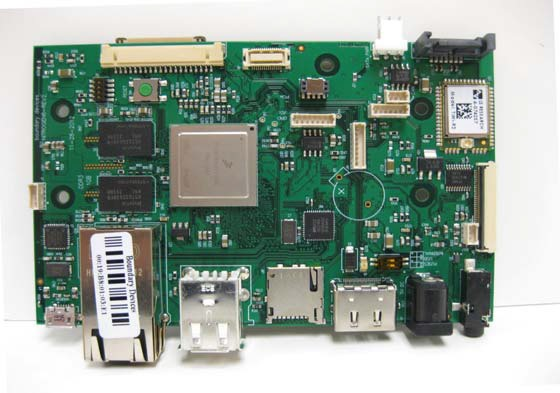
\includegraphics[]{figures/nitrogen6x}
	\caption{Nitrogen6X Development Kit \cite{nitrogen6x}}
	\label{fig:app:nitrogen6x}
\end{figure}
\newpage

\section{iMX6Quad CPU}
\label{app:imx6q}

\begin{figure}[h!]
	\centering
	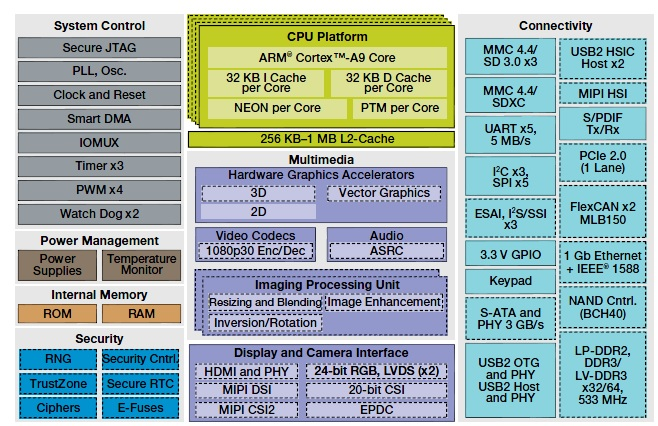
\includegraphics[width=160mm, height=110mm]{figures/imx6q}
	\caption{Internals of iMX6Quad CPU \cite{imx_spec}}
	\label{fig:app:imx6q}
\end{figure}

\cleardoublepage
\chapter{Description of the Benchmark Functions}
\label{description:benchmark}
\begin{longtable}{rp{120mm}}
	\hypertarget{benchmarks}{100CMYACC8:}& Multiply each element of a 100 x 8-element complex matrix with an 8-element complex vector and accumulate the 8 complex multiplication results to a single complex result, resulting in a 100 x 1-element complex matrix. \\[0.2cm]
	100RMY50: & Multiply each vector in a 100 x 50-element complex matrix with a 50-element float vector, resulting in a 100 x 50-element complex matrix.\\[0.2cm]
	100CONV64: & Perform fast convolution of a 100 x 64-element complex matrix: complex 64-pt FFT, followed by a multiplication with a 64-element float vector, followed by a 64-pt complex inverse FFT, resulting in a 100 x 64-element complex matrix. \\[0.2cm]
	150COT50: & Perform a corner turning of a 150 x 50 complex matrix into a 50 x 150 complex matrix incl. zero-padding of the elements from 150 to 256\\ [0.2cm]
	50MAG256: & Perform with a 50 x 256-element complex matrix a magnitude square-root calculation, resulting in a 50 x 256 float matrix. \\[0.2cm]
	64AVG100: & Calculate from a 64 x 100-element float matrix the average within a 5x5 area around the cell. Resulting in a 64 x 100-element float matrix. \\[0.2cm]
	64CMPR100: & Compare a 64 x 100-element float matrix with a float threshold. If  the threshold is exceeded, the corresponding element in a 64 x 100 boolean matrix shall be set to TRUE, otherwise set to FALSE. \\[0.2cm]
\end{longtable}
\cleardoublepage

%%%%%%%%%%%%%%%%%%%%%%%%%%%%%%%%%%%%%%%%%%%%%%%%%%%%%%%%%%%%%%%%%%%%%%%%%%
%%%%%%%%%%%%   CAPTER   %%%%%%%%%%%%%%%%%%%%%%%%%%%%%%%%%%%%%%%%%%%%%%%%%%
%%%%%%%%%%%%%%%%%%%%%%%%%%%%%%%%%%%%%%%%%%%%%%%%%%%%%%%%%%%%%%%%%%%%%%%%%%
\chapter{Code Snippets}
\label{app:code}

\section{set\_core\_affinity()}
\label{app:code:core_affinity}

\lstset{ %
  backgroundcolor=\color{mildyellow},
  basicstyle=\ttfamily\small,
  breakatwhitespace=false,
  breaklines=true,
  captionpos=b,
  commentstyle=\color{mygreen},
  keepspaces=true,
  keywordstyle=\color{blue},
  otherkeywords={cpu\_set\_t,pthread\_t},
  numbers=left,
  numberstyle=\tiny\color{mygray},
  frame=single,
  showspaces=false,
  showstringspaces=false,
  stringstyle=\color{mymauve},
  language=C
}

\begin{lstlisting}[caption=Set core affinity of calling thread]
int set_core_affinity(int core_id)
{
  int num_cores = sysconf(_SC_NPROCESSORS_ONLN);
  if (core_id < 0 || core_id >= num_cores)
    return CPU_AFFINITY_ERROR;

  cpu_set_t cpuset;
  CPU_ZERO(&cpuset);
  CPU_SET(core_id, &cpuset);

  pthread_t current_thread = pthread_self();
  if(pthread_setaffinity_np(current_thread, sizeof(cpu_set_t), &cpuset) != 0) 
    return CPU_AFFINITY_ERROR;

  return CPU_AFFINITY_OK;
}
\end{lstlisting}


\newpage
\section{wait\_for\_all\_threads()}
\label{app:code:wait_for_others}

\begin{lstlisting}[caption=Wait for other threads to join]
void wait_for_all_threads()
{
  while(awakenedThreads%NUM_THREADS != 0)
    sleep(0.001);

  pthread_mutex_lock(&mutex);
  readyThreads += 1;

  if(readyThreads == NUM_THREADS) {
    pthread_cond_broadcast(&cv_count);
  }

  while(readyThreads != NUM_THREADS)
    pthread_cond_wait(&cv_count, &mutex);

  ++awakenedThreads;
  if(awakenedThreads == NUM_THREADS){
    awakenedThreads = 0;
    readyThreads = 0;
  }

  pthread_mutex_unlock(&mutex);
}
\end{lstlisting}

\lstset{ %
  language=bash
}
\newpage
\section{mem\_util.sh}
\label{app:code:mem_util}
\begin{lstlisting}[caption=Peak Memory Utilization]
#!/bin/bash
ITER=1
PEAK_MEM=0
MEM_SIZE=`free -m | sed -n '2p'| awk '{print $2}'`
DATE_BEGIN=$(date +%Y-%m-%d" "%H:%M:%S)
OUTPUT_FILE="logs/peak_mem_util.csv"

echo "DATE BEGIN,${DATE_BEGIN}" > ${OUTPUT_FILE}

# Check for user input
if [ "$#" = "0" ]
then
# Read from file
PID=`cat logs/pid`
else
PID=$1
fi
echo "PID = ${PID}"

NAME=`cat /proc/${PID}/cmdline`
echo "Application name, ${NAME}" >> ${OUTPUT_FILE}
RES=`eval top -b -n ${ITER} | grep ${PID}`

while [ ! -z "$RES"  ]
do
#echo "res = ${RES}"
array=($RES)
PEAK_MEM=${array[9]}
echo "${PEAK_MEM}" >> ${OUTPUT_FILE}

#echo "Peak mem = ${PEAK_MEM}"
RES=`eval top -b -n ${ITER} | grep ${PID}`
sleep 0.1
done
\end{lstlisting}
\cleardoublepage

%%%%%%%%%%%%%%%%%%%%%%%%%%%%%%%%%%%%%%%%%%%%%%%%%%%%%%%%%%%%%%%%%%%%%%%%%%
%%%%%%%%%%%%   CAPTER   %%%%%%%%%%%%%%%%%%%%%%%%%%%%%%%%%%%%%%%%%%%%%%%%%%
%%%%%%%%%%%%%%%%%%%%%%%%%%%%%%%%%%%%%%%%%%%%%%%%%%%%%%%%%%%%%%%%%%%%%%%%%%
\chapter{Baseline Analysis Example Calculations}
\label{app:ba:calc:scheme1}

\section{Scheme-1}
\subsection{Utilization of Core\#1}
\begin{figure}[h!]
	\centering
	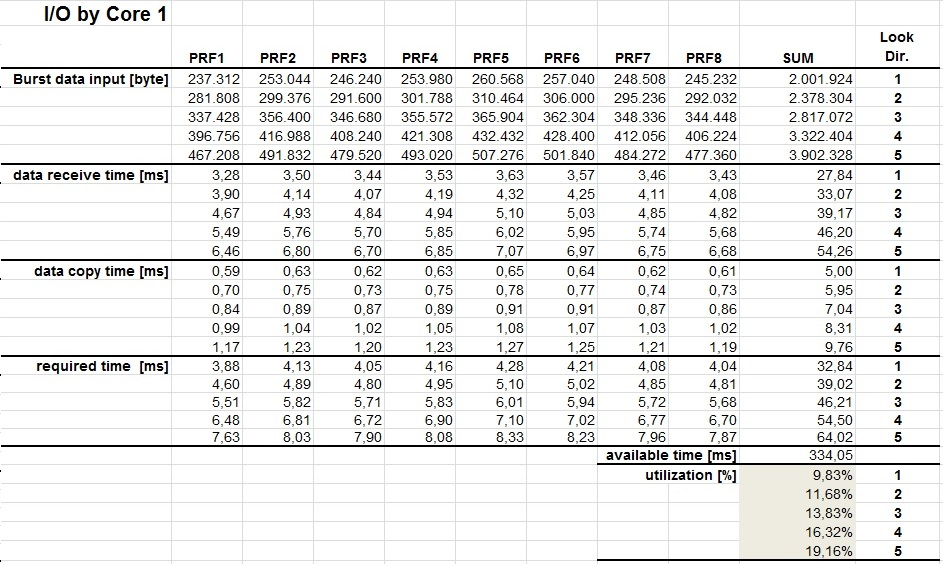
\includegraphics[width=150mm]{figures/aa_scheme1_cpu_util_1}
	\caption{Scheme-1, Core\#1 Utilization}
	\label{fig:existing_analysis:aa_scheme1_cpu_util1}
\end{figure}
\begin{align*}
	\label{aa:scheme1:core1:equ}
	Burst \enspace data \enspace input & = 64 pulses \enspace * \enspace 103 \frac{range gates}{pulse} \enspace * \enspace 9channel * 4\frac{byte}{sample}\\[0.3cm]
	& = 237,312 \enspace byte \\[0.3cm]
	Data \enspace receive \enspace time &= \frac{1}{19.5 \enspace * \enspace 10^{3} \enspace Hz} \enspace * \enspace 64 = 3.28 \enspace ms \\[0.3cm]
	Data \enspace copy \enspace time &= 237,312 byte \enspace * \enspace 2\frac{cycle}{byte} \enspace * \enspace 1.25\frac{ns}{cycle} = 0.59 \enspace ms \\[0.3cm]
	Required \enspace time &= 3.28ms + 0.59ms =  3.88ms\\[0.3cm]
	Available \enspace time &= 12 * min.dwelltime = 12*27.84ms = 334.05ms \stepcounter{equation}\tag{\theequation} 
\end{align*}

\subsection{Utilization of Core\#2}
\begin{figure}[h!]
	\centering
	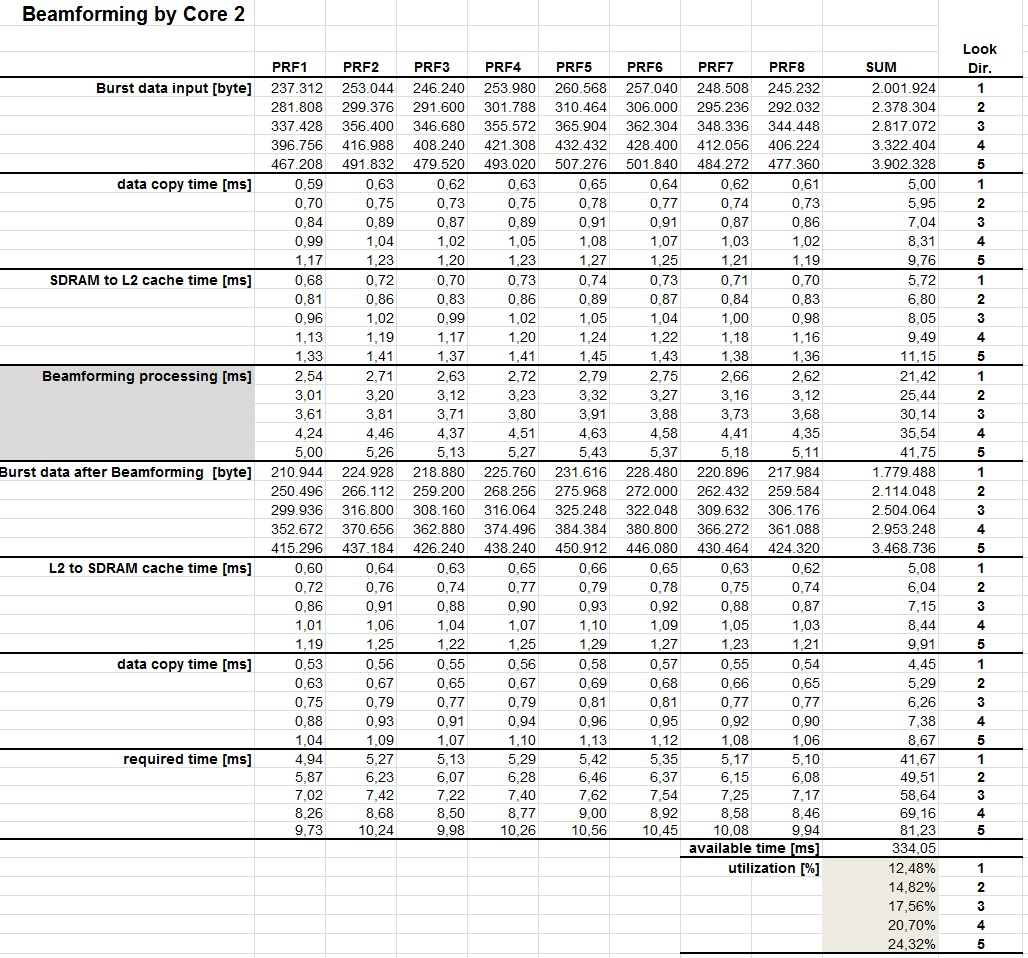
\includegraphics[width=150mm]{figures/aa_scheme1_cpu_util_2}
	\caption{Scheme-1, Core\#2 Utilization}
	\label{fig:existing_analysis:aa_scheme1_cpu_util2}
\end{figure}
\begin{align*}
\label{aa:scheme1:core2:equ1}
	SDRAM \: to \: L2cache \: time &= 237,312 byte \, * \, 2.29\frac{cycle}{byte} \, * \, 1.25\frac{ns}{cycle} = 0.68 \, ms \\[0.3cm]
	Beamforming \: processing &= 3channel * 64pulses * 103 \frac{range gates}{pulse} * 79\frac{cycle}{8 element} \\[0.3cm] 
	&\qquad * 1.25\frac{ns}{cycle} * 1.3(OSoverhead) = 2.54ms\\[0.3cm]
	Beamformed \: data &= 4channel * 64pulses * 103 \frac{range gates}{pulse} *8\frac{byte}{sample} = 210,944byte \\[0.3cm]
	L2cache \: to \: SDRAM \: time &= 210,944 byte \, * \, 2.29\frac{cycle}{byte} \, * \, 1.25\frac{ns}{cycle} = 0.60 \, ms \\[0.3cm]
	Data \: copy \: time &= 210,944 byte \, * \, 2.2\frac{cycle}{byte} \, * \, 1.25\frac{ns}{cycle} = 0.53 \, ms \\[0.3cm]
	Required \: time &= 0.59ms + 0.68ms + 2.54ms + 0.60ms + 0.53ms = 4.94ms \stepcounter{equation}\tag{\theequation} 
\end{align*}


\subsection{Utilization of Core\#3}
\begin{figure}[h!]
	\centering
	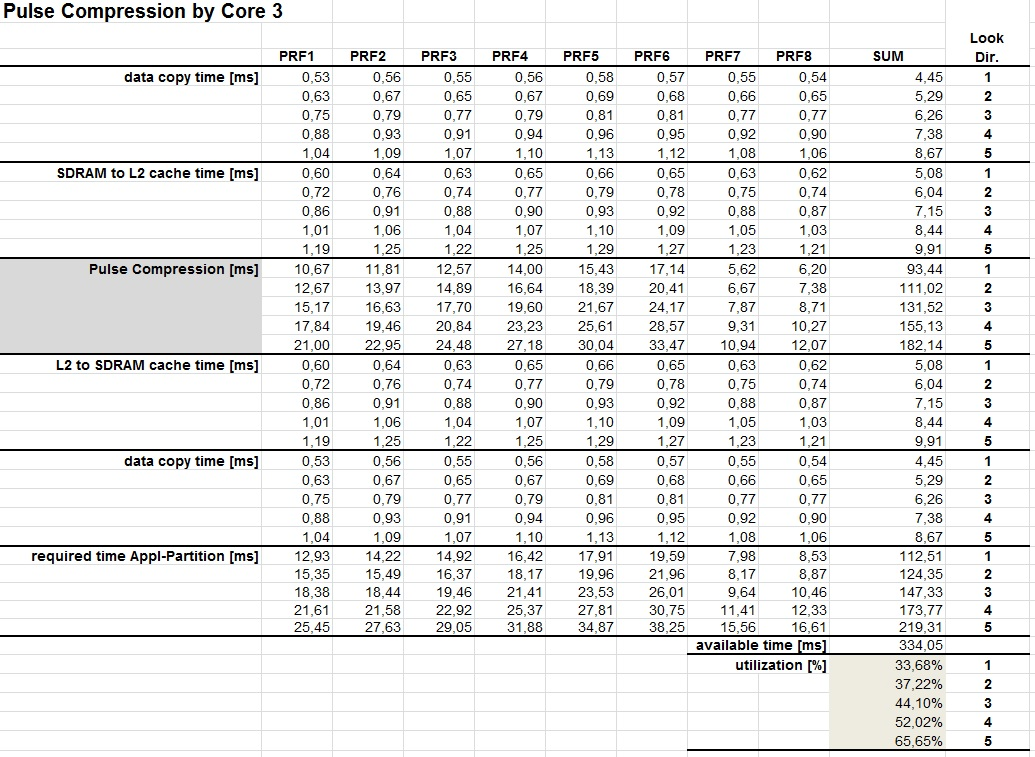
\includegraphics[width=160mm]{figures/aa_scheme1_cpu_util_3}
	\caption{Scheme-1, Core\#3 Utilization}
	\label{fig:existing_analysis:aa_scheme1_cpu_util3}
\end{figure}
\begin{align*}
	\label{aa:scheme1:core3:equ}
	Pulse \: compression &= \bigg(\#channel * \#pulses (CONV128 +  \# \frac{range gates}{pulse} * RMY50)\bigg)\\[0.3cm]  
	& \quad * \# \: cycle \: time * OSoverhead\\[0.3cm] 
	&= (4 * 64 (24100 + 103 * 15)) * 1.25 * 1.3 = 10.67ms   \stepcounter{equation}\tag{\theequation} 
\end{align*}

\FloatBarrier
\subsection{Utilization of Core\#4}
\begin{align*}
	\label{aa:scheme1:core4:equ1}
	FDP \: time &= \bigg(4channel * (\#pulses * \# \frac{RG}{pulse} (COT50 + RMY50) + \# \frac{RG}{pulse} * FFT64) \\[0.3cm] 
	& \qquad + 2 * (\# \frac{range gates}{pulse} * 64 * MAG256)\bigg) * OSoverhead * cycle \, time \\[0.3cm]
	&= (4 * (64 * 103 (12 + 15) + 103 * 2550) + 2 * (103 * 64 * 20)) * 1.3 * 1.25ns \enspace \\[0.3cm]
	&= \enspace 3.29ms  \stepcounter{equation}\tag{\theequation} 
\end{align*}

\begin{figure}[h!]
	\centering
	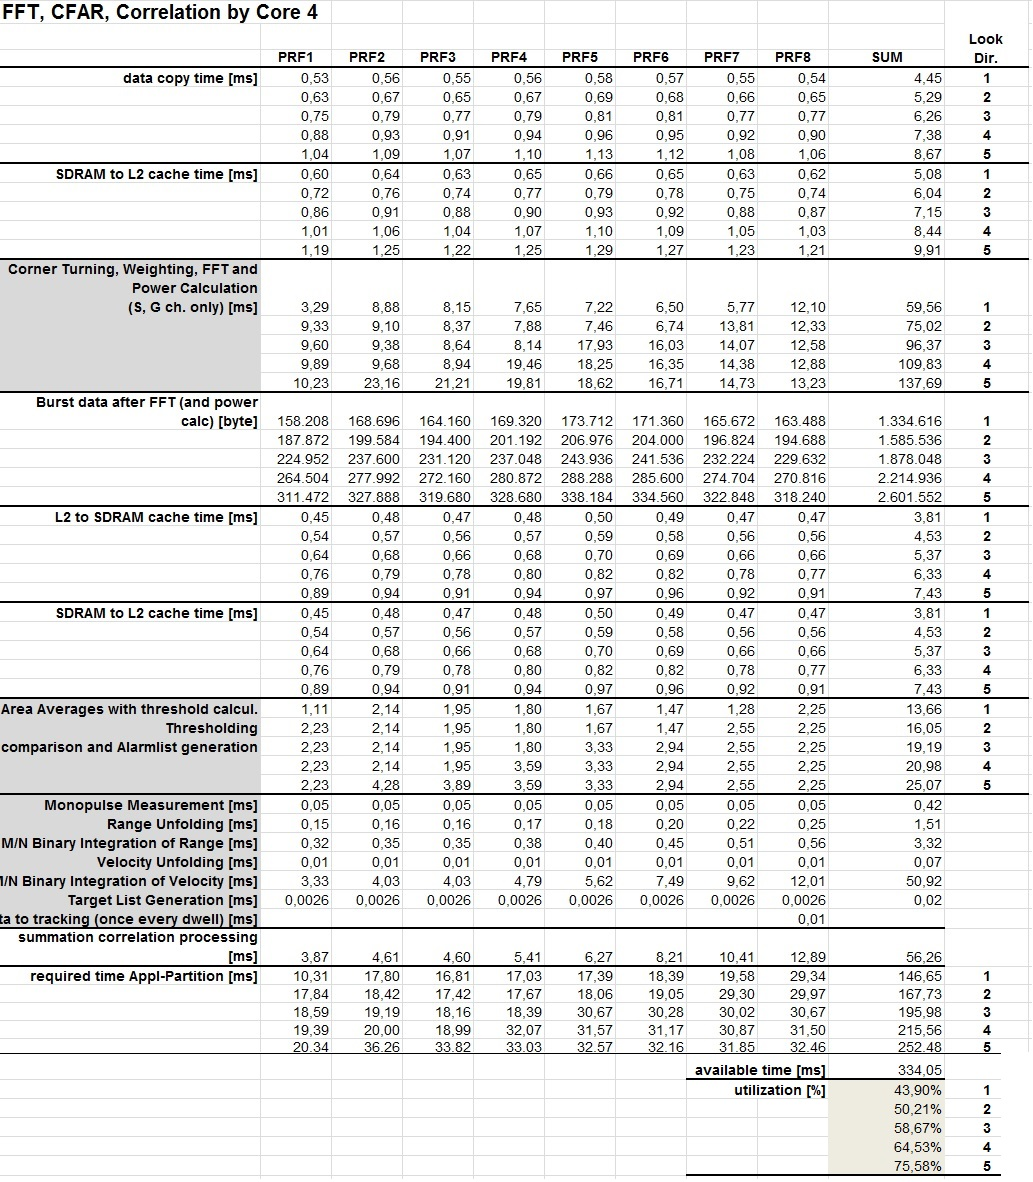
\includegraphics[width=150mm]{figures/aa_scheme1_cpu_util_4}
	\caption{Scheme-1, Core\#4 Utilization}
	\label{fig:existing_analysis:aa_scheme1_cpu_util4}
\end{figure}

\begin{align*}
	\label{aa:scheme1:core4:equ2}
		Data \: size \: after \: FDP &=  64pulses * 103 \frac{range gates}{pulse} ( 2 * 8 + 2 * 4) = 158,208 \: byte\\[0.25cm] 
		L2cache \: to \: SDRAM &= 158,208 byte \, * \, 2.29\frac{cycle}{byte} \, * \, 1.25\frac{ns}{cycle} = 0.45 \, ms \\[0.25cm]
		Average \: Calculation &= 2channel * 103 \frac{range gates}{pulse} * 64(FFTsize) * 20(AVG100) * 2 \\
		&=  527,360 \: cycle \\[0.25cm]
		Comparison &= 2channel * 103 \frac{range gates}{pulse} * 64(FFTsize) * 7(CMPR100) \\
		&= 92,288 \: cycle \\[0.25cm]
		Detection &= 1channel * 103 \frac{range gates}{pulse} * 64(FFTsize) * 10(DET100) \\
		&= 65,920 \: cycle \\[0.25cm]
		Time \: required &= (Average \, calculation + Comparison + Detection) \\
		& \qquad * OSoverhead * cycle \, time \\[0.25cm]
		&= (527,360 + 92,288 + 65,920) * 1.3 * 1.25ns = 1.1ms \stepcounter{equation}\tag{\theequation} 
\end{align*}

\begin{align*}
	\label{aa:scheme1:core4:equ3}
		Monopulse \: Measurement &= 2channel * \#\frac{alarms}{burst} * \#\frac{cycle}{alarm} * OSoverhead * cycle \: time \\
		&= 2 * 32 * 500 * 1.3 * 1.25ns = 0.05 \: ms \\
		Range \: Unfolding &= \bigg(RG_{max} * \#\frac{cycle}{rangegate} + \# Unfoldings * \#\frac{alarms}{burst} * \#cycle\bigg) \\
		& \qquad *OSoverhead * cycle \: time \\
		&= (987 * 30 + 10 * 32 * 200) * 1.3 * 1.25ns = 0.15 \: ms \\
		M/N \: Range \: Integration &= \bigg(\#RangeGates * \#\frac{cycle}{rangegate} + \#Unfoldings * \#\frac{alarms}{burst} \\
		&\qquad * \#\frac{cycle}{alarm}\bigg) * OSoverhead *cycle \: time \\
		&= (988 * 40 + 32 * 10 * 500) * 1.3 * 1.25ns = 0.32 \: ms \\
		Velocity \: Unfolding &= \bigg(\#Unfoldings * \#\frac{alarms}{burst} * \#\frac{cycle}{alarm}\bigg) \\
		& \qquad * OSoverhead * \#cycle \: time \\
		&= (8 * 32 * 30) * 1.3 * 1.25ns = 0.01 \: ms \\
		M/N \: Velocity \: Integration &= \bigg(\#\frac{alarms}{burst} * \#Unfoldings^{2} * \#bursts * \#\frac{cycle}{alarm}\bigg) \\
		& \qquad * OSoverhead * cycle \: time \\
		&= (32 * 10^{2} * 8 * 80) * 1.3 * 1.25ns =  3.33 \: ms \\
		Target \: List \: Generation &= \bigg(\#targets * \#\frac{cycle}{target}\bigg) * OSoverhead * cycle \: time \\
		&= (16 * 100) * 1.3 * 1.25ns = 0.0026 \: ms \\
		Correlation \: Processing[ms] &= 0.05 + 0.15 + 0.32 + 0.01 + 3.33 + 0.0026 = 3.87 \: ms \\
		Required \: time[ms] &= 0.53 + 0.60 + 3.29 + 0.45 + 0.45 + 0.11 + 3.87 = 10.31 \: ms \stepcounter{equation}\tag{\theequation}
\end{align*}

\subsection{Processing Latency}
\label{app:sch1:proc_late}
\begin{align*}
	\label{aa:scheme1:latency}
		Processing \: latency &= IO + Beamforming + Pulse \: compression  + FFT,CFAR,Correlation \\
		&= 32.84 + 41.67 + 112.51 + 146.65 = 333.67 \: ms \\[0.3cm]
		\#Dwells \: transmitted &= \frac{processing \: latency}{dwell \: time} = \frac{333.67}{27.84} = 11.99 \stepcounter{equation}\tag{\theequation}
\end{align*}

\subsection{Memory Utilization}
\label{app:sch1:mem_util}
\begin{figure}[h!]
	\centering
	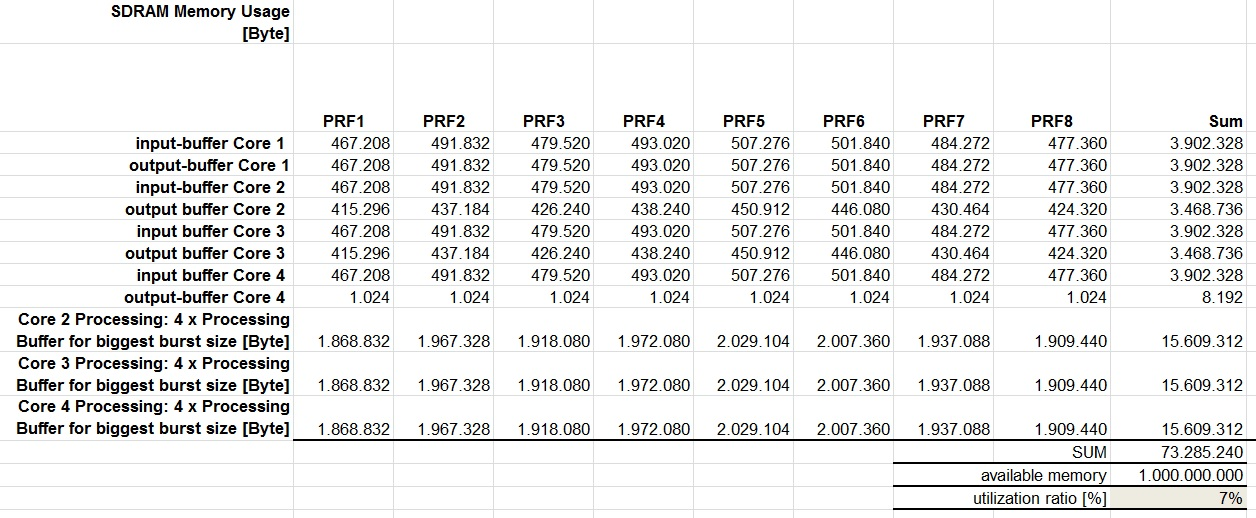
\includegraphics[width=160mm]{figures/aa_scheme1_mem_util}
	\caption{Scheme-1, Memory Utilization}
	\label{fig:existing_analysis:aa_scheme1_mem_util}
\end{figure}

\subsection{Interface Utilization}
\label{app:sch1:mem_util}
The DGPMs are identical, thus only one DGPM's utilization is listed here.
\begin{figure}[h!]
	\centering
	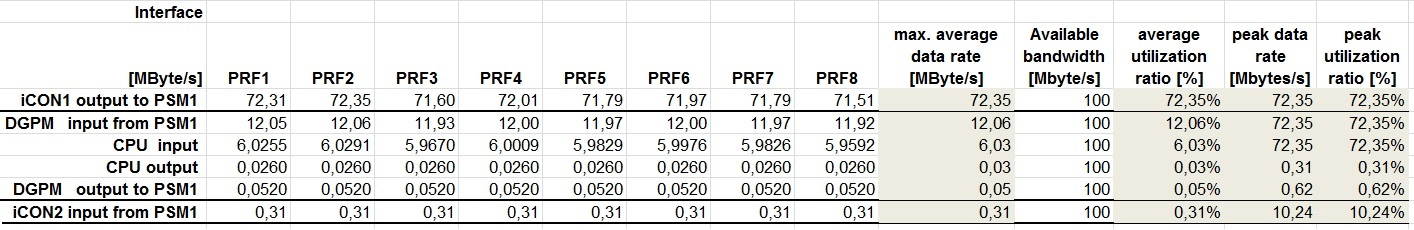
\includegraphics[width=160mm]{figures/aa_scheme1_interface_util}
	\caption{Scheme-1, Interface Utilization}
	\label{fig:existing_analysis:aa_scheme1_interface_util}
\end{figure}
\begin{align*}
	\label{equ:aa:scheme1:interface_util}
	iCON1 \: output \: to \: PSM1 &= \#\frac{byte}{sample} * \#channel * range \: gate * frequency \\
	&= 4 * 9 * 103 * 19.5kHz = 72.31 \: MB/s \\
	DGPM \: input \: from \: PSM &= \frac{data \: rate}{\#DGPMs} = \frac{72.31}{6} = 12.05 \: MB/s \\[0.3cm]
	CPU \: input &= \frac{DGPM \: data \: rate}{\#CPUs} = \frac{12.05}{2} = 6.02 \: MB/s \\[0.3cm]
	DGPM \: output \: to \: PSM &= \frac{data \: rate}{\#DGPMs} = \frac{0.31}{6} = 0.0526 \: MB/s \\[0.3cm]
	CPU \: output &= \frac{DGPM \: output}{\#CPUs} = \frac{0.0526}{2} = 0.026 \: MB/s \stepcounter{equation}\tag{\theequation}
\end{align*}

\chapter{Scheme-3 Calculations}
\label{app:sch3:calc}

\section{IO Processing}
\begin{figure}[h!]
	\centering
	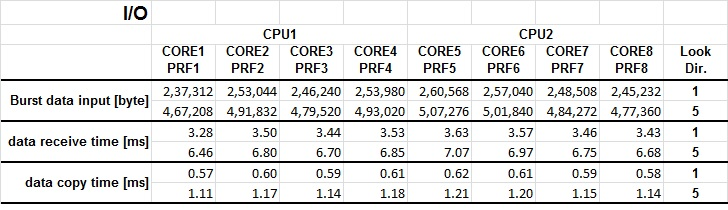
\includegraphics[width=140mm]{figures/scheme4_io}
	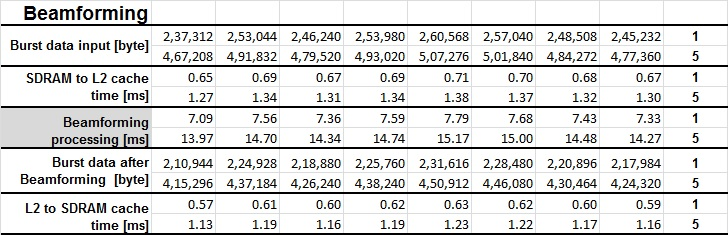
\includegraphics[width=140mm]{figures/scheme4_bf}
	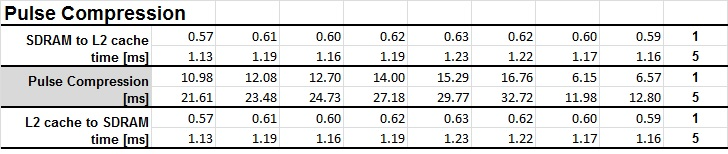
\includegraphics[width=140mm]{figures/scheme4_pc}
	\caption{Scheme-3, Input Output, Beamforming and Pulse Compression}
	\label{fig:mm:scheme4_io}
\end{figure}

\section{FFT and CFAR Processing}
\FloatBarrier
\begin{figure}[h!]
	\centering
	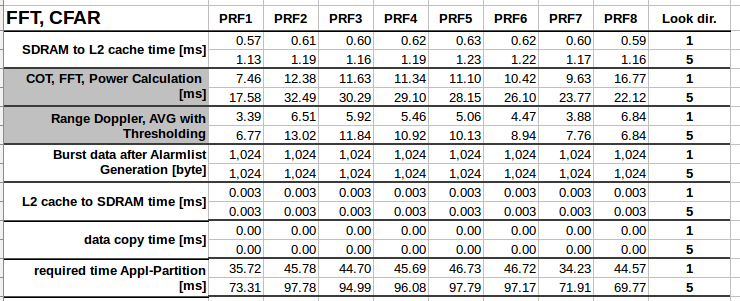
\includegraphics[width=140mm]{figures/scheme4_fft}
	\caption{Scheme-3, FFT and CFAR Processing}
	\label{fig:mm:scheme4_fft}
\end{figure}

\section{CPU Utilization}
\label{app:sch3:cpu_util}
\begin{figure}[h!]
	\centering
	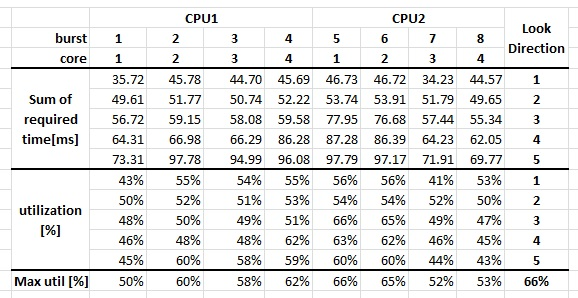
\includegraphics[width=140mm]{figures/scheme4_util}
	\caption{Scheme-3, CPU Utilization}
	\label{fig:mm:scheme4_util}
\end{figure}